\chapter{Methodology}  %Title of the First Chapter

\ifpdf
    \graphicspath{{Chapter4/Figs/Raster/}{Chapter4/Figs/PDF/}{Chapter4/Figs/}}
\else
    \graphicspath{{Chapter4/Figs/Vector/}{Chapter4/Figs/}}
\fi

%\section{Methodology}
%\label{sec:method}

\section{Datasets}

2018 luminosity data taking is divided into seven periods namely A, B, C, D1, D2, D3 and D4 as shown in Fig. \ref{fig:period_bound}. vdM data is shown during period B corresponding to Fill 6868. Run range for each period is shown in Table \ref{tab:period run ranges}. 

\begin{figure}[!htp]
\centering
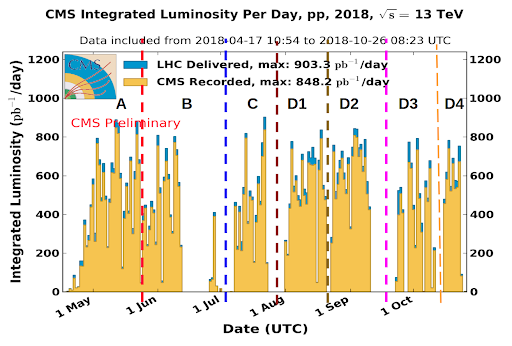
\includegraphics[width=0.8\textwidth]{ashish_thesis/period_boundary.png}
\caption{%
   2018 luminosity data taking periods showing data taking period boundaries and vdM calibration data.
}
\label{fig:period_bound}
\end{figure}


\begin{table}[htbp]
  \centering
  \begin{tabular}{@{}c@{\hspace{1cm}}p{5.5cm}p{5.5cm}@{}}
    \textbf{Period} & \textbf{Random Trigger Dataset} & \textbf{Zero Bias Dataset} \\
    2018A & \begin{tabular}{@{}p{5.5cm}@{}}/AlCaLumiPixels/Run2018A-AlCaPCCRandom-15Apr2023\_UL2018\_315252\_316062\_PCCRandom\_-v1/ALCARECO, \\ /StreamALCALUMIPIXELSEXPRESS/Run2018A-AlCaPCCRandom-Express-v1/ALCARECO\end{tabular} & /AlCaLumiPixels/Run2018A-AlCaPCCZeroBias-13Mar2023\_UL2018\_PCC-v1/ALCARECO \\
    2018B & /StreamALCALUMIPIXELSEXPRESS/Run2018B-AlCaPCCRandom-Express-v1/ALCARECO & /AlCaLumiPixels/Run2018B-AlCaPCCZeroBias-13Mar2023\_UL2018\_PCC-v1/ALCARECO \\
    2018C & /StreamALCALUMIPIXELSEXPRESS/Run2018C-AlCaPCCRandom-Express-v1/ALCARECO & /AlCaLumiPixels/Run2018C-AlCaPCCZeroBias-13Mar2023\_UL2018\_PCC-v1/ALCARECO \\
    2018D & /StreamALCALUMIPIXELSEXPRESS/Run2018D-AlCaPCCRandom-Express-v1/ALCARECO & /AlCaLumiPixels/Run2018D-AlCaPCCZeroBias-PromptReco-v2/ALCARECO \\
  \end{tabular}
  \caption{Dataset Information}
  \label{tab:datasets}
\end{table}

\textbf{/AlCaLumiPixels/Run2018A-AlCaPCCRandom15Apr2023\_UL2018\_315252\_316062\_PCCRandom\_-v1/ALCARECO} 

%\textbf{/AlCaLumiPixels/Run2018A-AlCaPCCRandom15Apr2023_UL2018_315252_316062_PCCRandom_-v1/ALCARECO}

\begin{itemize}

\item /AlCaLumiPixels/Run2018A: This indicates that the dataset is related to the "AlCa" (ALignment and CALibration) stream, specifically for the "LumiPixels" subdetector. The data corresponds to the Run2018A period, which means it was collected during the first run period in 2018.

\item AlCaPCCRandom: This tag represents the primary dataset and the trigger path used to collect the data. "PCC" stands for "Pixel Cluster Counting" and is a method for luminosity measurement. "Random" indicates that this dataset was collected using a random trigger, which is a method to sample a fraction of the events by applying trigger on both colliding and non-colliding bunch crossings.

\item $15Apr2023_UL2018_315252_316062_PCCRandom_-v1$: This part represents the processing version, date, and run range of the dataset. "15Apr2023" is the date when this specific version of the dataset was created. "UL2018" indicates that this data has been processed using the "Ultra Legacy" (UL) campaign for the 2018 dataset, which aims to provide the highest quality data for physics analysis. The numbers $"315252_316062"$ represent the range of run numbers included in the dataset. $"PCCRandom_"$ is a reference to the Pixel Cluster Counting method used for luminosity measurement and the random trigger. "v1" denotes the version number of this processed dataset.

\item ALCARECO:
This acronym stands for "ALignment and CALibration RECOstruction." It is a data tier representing the output of specific reconstruction algorithms applied to the raw data to produce high-level objects needed for the alignment and calibration tasks.

\end{itemize}

%To summarize, this dataset is a collection of events from the CMS experiment during the Run2018A period, sampled using a random trigger. It is specifically related to the luminosity measurement using the Pixel Cluster Counting method. The dataset has been processed using the Ultra Legacy campaign, and the output contains high-level objects required for alignment and calibration tasks.



$\textbf{/StreamALCALUMIPIXELSEXPRESS/Run2018A-AlCaPCCRandom-Express-v1/ALCARECO}$

\begin{itemize}

\item /StreamALCALUMIPIXELSEXPRESS/Run2018A:
This indicates that the dataset is related to the "AlCa" (ALignment and CALibration) stream, specifically for the "LumiPixels" subdetector, and is part of the "Express" data processing tier. The data corresponds to the Run2018A period, which means it was collected during the first run period in 2018.

\item AlCaPCCRandom:
This tag represents the primary dataset and the trigger path used to collect the data. "PCC" stands for "Pixel Cluster Counting" and is a method for luminosity measurement. "Random" indicates that this dataset was collected using a random trigger, which is a method to sample a fraction of the events without specific selection criteria (i.e., unbiased events).

\item Express-v1:
This part represents the processing version and the type of data processing. "Express" indicates that this data has been processed using the "Express" campaign, which is a near-real-time processing of the data as it is collected. This type of processing is essential for providing timely feedback to the experiments and enabling rapid identification of any issues. "v1" denotes the version number of this processed dataset.

\item ALCARECO:
This acronym stands for "ALignment and CALibration RECOstruction." It is a data tier representing the output of specific reconstruction algorithms applied to the raw data to produce high-level objects needed for the alignment and calibration tasks.

\end{itemize}

%In summary, this dataset is a collection of events from the CMS experiment during the Run2018A period, sampled using a random trigger. It is specifically related to the luminosity measurement using the Pixel Cluster Counting method. The dataset has been processed using the Express campaign, and the output contains high-level objects required for alignment and calibration tasks.


%$\textbf{/AlCaLumiPixels/Run2018A-AlCaPCCZeroBias-13Mar2023_UL2018_PCC-v1/ALCARECO}$

$\textbf{/AlCaLumiPixels/Run2018A-AlCaPCCZeroBias-13Mar2023\_UL2018\_PCC-v1/ALCARECO}$

\begin{itemize}

\item /AlCaLumiPixels/Run2018A:
This indicates that the dataset is related to the "AlCa" (ALignment and CALibration) stream, specifically for the "LumiPixels" subdetector. The data corresponds to the Run2018A period, which means it was collected during the first run period in 2018.

\item AlCaPCCZeroBias:
This tag represents the primary dataset and the trigger path used to collect the data. "PCC" stands for "Pixel Cluster Counting" and is a method for luminosity measurement. "ZeroBias" indicates that this dataset was collected using a trigger with no specific selection criteria (i.e., unbiased events).

\item $13Mar2023_UL2018_PCC-v1$:
This part represents the processing version and the date of the dataset. "13Mar2023" is the date when this specific version of the dataset was created. "UL2018" indicates that this data has been processed using the "Ultra Legacy" (UL) campaign for the 2018 dataset, which aims to provide the highest quality data for physics analysis. "PCC" is again a reference to the Pixel Cluster Counting method used for luminosity measurement. "v1" denotes the version number of this processed dataset.

\item ALCARECO:
This acronym stands for "ALignment and CALibration RECOstruction." It is a data tier representing the output of specific reconstruction algorithms applied to the raw data to produce high-level objects needed for the alignment and calibration tasks.


\end{itemize}

%So, to summarize, this dataset is a collection of unbiased events from the CMS experiment during the Run2018A period. It is specifically related to the luminosity measurement using the Pixel Cluster Counting method. The dataset has been processed using the Ultra Legacy campaign, and the output contains high-level objects required for alignment and calibration tasks.


$\textbf{/AlCaLumiPixels/Run2018D-AlCaPCCZeroBias-PromptReco-v2/ALCARECO}$

\begin{itemize}

\item /AlCaLumiPixels/Run2018D:
This indicates that the dataset is related to the "AlCa" (ALignment and CALibration) stream, specifically for the "LumiPixels" subdetector. The data corresponds to the Run2018D period, which means it was collected during the fourth run period in 2018.

\item AlCaPCCZeroBias:
This tag represents the primary dataset and the trigger path used to collect the data. "PCC" stands for "Pixel Cluster Counting" and is a method for luminosity measurement. "ZeroBias" indicates that this dataset was collected using a trigger with no specific selection criteria (i.e., unbiased events).

\item PromptReco-v2:
This part represents the processing version and the type of data processing. "PromptReco" indicates that this data has been processed using the "Prompt Reconstruction" campaign, which is a near-real-time processing of the data as it is collected. This type of processing is essential for providing timely feedback to the experiments and enabling rapid identification of any issues. "v2" denotes the version number of this processed dataset.

\item ALCARECO:
This acronym stands for "ALignment and CALibration RECOstruction." It is a data tier representing the output of specific reconstruction algorithms applied to the raw data to produce high-level objects needed for the alignment and calibration tasks.

\end{itemize}

%In summary, this dataset is a collection of unbiased events from the CMS experiment during the Run2018D period, specifically related to the luminosity measurement using the Pixel Cluster Counting method. The dataset has been processed using the Prompt Reconstruction campaign, and the output contains high-level objects required for alignment and calibration tasks.






























\begin{comment}


The dataset /StreamALCALUMIPIXELSEXPRESS/Run2018A-AlCaPCCRandom-Express-v1/ALCARECO, is a dataset from the CMS experiment at CERN's Large Hadron Collider (LHC). This dataset is specifically collected for luminosity measurements using pixel cluster counting (PCC) in the CMS detector by applying trigger on colliding and non-colliding bunches. 

\begin{itemize}

\item StreamALCALUMIPIXELSEXPRESS: This indicates that the dataset is related to the "AlCa" (Alignment and Calibration) sub-system of the CMS detector, specifically focused on luminosity measurements using the pixel detector. The "EXPRESS" in the name signifies that this dataset is processed using the Express Stream, which is a fast data processing system for near real-time analysis of CMS data.

\item Run2018A: This represents the run period during which the data was collected. In this case, it refers to the 2018 data-taking period, specifically the "A" run.

\item AlCaPCCRandom: This indicates that the dataset is related to the "PCC" (Pixel Cluster Counting) method of luminosity measurement, and "Random" refers to the trigger used for data collection. In this case, a random trigger is used, selecting events without any specific bias.

\item Express-v1: This signifies that the dataset has been processed using the Express Stream system. The "-v1" indicates the version of the processing.

\item ALCARECO: This is the final data format of the dataset, specifically designed for alignment and calibration tasks.

%\item Data collection: The CMS detector collects data from proton-proton collisions at the LHC. For this dataset, a random trigger is used , ensuring a representative sample of events for luminosity measurements.

%\item Data processing: The raw data is processed using the Express Stream system. This is a fast processing system used for near real-time analysis of CMS data. During this process, the raw data is converted into higher-level objects, such as tracks and vertices, which are more convenient for analysis.

%\item Data filtering: ALCARECO datasets are created by applying specific filters and selections to the processed data. In this case, the filters are chosen to focus on pixel cluster counting for luminosity measurements.

%\item Dataset storage: The final ALCARECO dataset is stored and made available for analysis by researchers working on alignment, calibration, and luminosity-related studies.

\end{itemize}


 The dataset /AlCaLumiPixels/Run2018D-AlCaPCCZeroBias-PromptReco-v2/ALCARECO, is specifically collected for luminosity measurements using pixel cluster counting (PCC) in the CMS detector by applying trigger on only colliding bunches. 

\begin{itemize}

\item AlCaLumiPixels: This indicates that the dataset is related to the "AlCa" (Alignment and Calibration) sub-system of the CMS detector, specifically focused on luminosity measurements using the pixel detector.

\item Run2018A: This represents the run period during which the data was collected. In this case, it refers to the 2018 data-taking period, specifically the "A" run.

\item AlCaPCCZeroBias: This indicates that the dataset is related to the "PCC" (Pixel Cluster Counting) method of luminosity measurement, and "ZeroBias" refers to the trigger used for data collection. ZeroBias triggers are unbiased, meaning they are randomly triggered and do not rely on any specific event characteristics.

\item PromptReco-v2: This signifies that the dataset has been processed using the "PromptReco" (Prompt Reconstruction) system, which is a fast processing system for real-time analysis of CMS data. The "-v2" indicates the version of the processing.

\item ALCARECO: This is the final data format of the dataset, specifically designed for alignment and calibration tasks.

%\item Data collection: The CMS detector collects data from proton-proton collisions at the LHC. For this dataset, the ZeroBias trigger is used, ensuring an unbiased sample of events for luminosity measurements.

%\item Data processing: The raw data is processed using the Prompt Reconstruction system. During this process, the raw data is converted into higher-level objects, such as tracks and vertices, which are more convenient for analysis.

%\item Data filtering: ALCARECO datasets are created by applying specific filters and selections to the processed data. In this case, the filters are chosen to focus on pixel cluster counting for luminosity measurements.

%\item Dataset storage: The final ALCARECO dataset is stored and made available for analysis by researchers working on alignment, calibration, and luminosity-related studies.

\end{itemize}

The dataset "AlCaLumiPixels/Run2018D-AlCaPCCZeroBias-PromptReco-v2/ALCARECO" dataset is a specialized dataset that provides information related to luminosity measurements using pixel detectors.

\begin{itemize}

\item AlCaLumiPixels: The term "AlCaLumiPixels" indicates that the dataset focuses on luminosity measurements obtained from the pixel detectors. The pixel detectors are part of the CMS experiment's innermost layers and are designed to precisely track the paths of charged particles produced in proton-proton collisions.

\item Run2018D: The "Run2018D" refers to a specific data-taking period or run period of the CMS experiment. The LHC operates in cycles of data-taking known as runs, which are typically identified by a year and a letter. In this case, "2018D" corresponds to a particular period of data collection in 2018.

\item AlCaPCCZeroBias: "AlCaPCCZeroBias" is a term that likely indicates the specific algorithm and event type used for luminosity measurement. The "PCC" stands for "Pixel Cluster Counting," which is an algorithm employed to estimate the instantaneous luminosity based on the information recorded by the pixel detectors. The "ZeroBias" events represent a special category of collisions where all the CMS detector systems trigger, regardless of the specific physics processes involved. These events are particularly useful for luminosity measurements.

\item PromptReco-v2: "PromptReco" refers to the reconstruction process for the prompt data. Prompt reconstruction involves the real-time processing and calibration of the recorded data immediately after it is taken. The "-v2" indicates a specific version or iteration of the prompt reconstruction process.

\item ALCARECO: "ALCARECO" stands for "ALignment CALibration RECOnditioned" data. It is a category of specialized reconstructed datasets produced with specific requirements for alignment and calibration studies. These datasets are carefully processed and conditioned to ensure accurate alignment of the CMS detector elements and precise calibration of the recorded data.

\end{itemize}


PromptReco (Prompt Reconstruction) and AlCaReco (ALignment and CALibration REConstructed Objects) are two different data processing and formatting systems used in the CMS experiment at CERN's Large Hadron Collider (LHC). While both systems are related to the processing of data collected by the CMS detector, they serve different purposes and have distinct features. Here is a comparison of the two systems:

Purpose: \\ 
PromptReco: The primary goal of the PromptReco system is to rapidly convert the raw data collected by the CMS detector into a format more suitable for physics analysis. It reconstructs the raw data into higher-level objects like tracks, vertices, and calorimeter clusters, which are then used by researchers to study various aspects of the particle collisions.

AlCaReco: The main purpose of the AlCaReco system is to provide specialized datasets for detector alignment, calibration, and other related tasks. AlCaReco datasets are generated by applying specific filters and selections to the reconstructed data (RECO), focusing on events and information that are particularly useful for alignment, calibration, and performance monitoring.

Data format: \\
PromptReco: The output of the PromptReco system is the RECO (REConstructed Objects) data format. This is the primary data format used for physics analysis in the CMS experiment, containing reconstructed objects such as tracks, vertices, and calorimeter clusters.

AlCaReco: The AlCaReco data format is designed specifically for alignment, calibration, and performance monitoring tasks. It is a more focused and compact data format, containing only the events and information relevant to the specific task, resulting in reduced data volume compared to the full RECO data.

Data processing:\\
PromptReco: The PromptReco system processes the raw data at Tier-0 of the Worldwide LHC Computing Grid (WLCG), using a series of algorithms to reconstruct the detector information into higher-level physics objects.

AlCaReco: The AlCaReco processing stream is applied after the PromptReco system, using the reconstructed data (RECO) as input. AlCaReco datasets are generated by applying specific filters and selections tailored to the needs of the alignment, calibration, and performance monitoring tasks.

%The main difference between PromptReco and AlCaReco is their purpose and the type of data they produce. PromptReco is focused on the rapid reconstruction of raw data into a format suitable for physics analysis, while AlCaReco is designed to provide specialized datasets for detector alignment, calibration, and performance monitoring tasks. Both systems play a crucial role in the overall data processing and analysis pipeline of the CMS experiment.

%AlCaReco stands for "ALignment and CALibration REConstructed Objects." It is a specific data format and processing stream used by the CMS experiment at CERN's Large Hadron Collider (LHC) for the purpose of detector alignment, calibration, and other specialized tasks. AlCaReco datasets are designed to be smaller and more focused compared to the primary reconstructed data (RECO), making them suitable for specialized analyses that require a specific set of event characteristics or detector information. The AlCaReco data format and processing stream serve several important functions: Customized event selection: AlCaReco datasets are generated by applying specific filters and selections to the reconstructed data (RECO). These filters are tailored to select events that are particularly useful for alignment, calibration, and other specialized tasks. For example, certain triggers or event topologies might be more suitable for studying the performance of a specific detector subsystem or measuring certain quantities. By selecting events with these specific characteristics, the AlCaReco datasets provide a more focused sample for the targeted analyses. Reduced data volume: One of the main advantages of AlCaReco datasets is their reduced data volume compared to the full RECO data. By selecting only the events and information relevant to the specific task, the AlCaReco data format helps save storage space and computational resources, making the data processing and analysis more efficient. Detector performance monitoring: AlCaReco datasets are used to monitor the performance of the CMS detector and its subsystems. By analyzing the data in these specialized datasets, researchers can track the detector's performance over time and identify any potential issues or areas for improvement. This information can then be used to optimize the detector's operation and ensure accurate data collection. Alignment and calibration: Accurate detector alignment and calibration are crucial for the overall performance of the CMS experiment. AlCaReco datasets provide the necessary information to perform these tasks, allowing researchers to refine the detector's geometry, timing, and energy response. This, in turn, improves the quality of the data collected by the CMS detector and increases the accuracy of the physics analyses. In summary, AlCaReco is a specialized data format and processing stream used by the CMS experiment for tasks related to detector alignment, calibration, and performance monitoring. By providing focused datasets with reduced data volume, AlCaReco enables efficient and accurate analysis of the data needed to maintain and optimize the performance of the CMS detector. AlCaReco: The main purpose of the AlCaReco system is to provide specialized datasets for detector alignment, calibration, and other related tasks. AlCaReco datasets are generated by applying specific filters and selections to the reconstructed data (RECO), focusing on events and information that are particularly useful for alignment, calibration, and performance monitoring. AlCaReco: The AlCaReco data format is designed specifically for alignment, calibration, and performance monitoring tasks. It is a more focused and compact data format, containing only the events and information relevant to the specific task, resulting in reduced data volume compared to the full RECO data. AlCaReco: The AlCaReco processing stream is applied after the PromptReco system, using the reconstructed data (RECO) as input. AlCaReco datasets are generated by applying specific filters and selections tailored to the needs of the alignment, calibration, and performance monitoring tasks.

\end{comment}

The calibration of luminosity measurement by the CMS experiment in the 2018 proton-proton data taking at $\sqrt{s}$ = 13 TeV was performed during

\begin{itemize}
\item LHC fill 6868 on June 30 and July 1, 2018 at $\sqrt{s}$ = 13 TeV
\item Zero-bias triggers on 5 bunch pairs (BCIDs 265, 865, 1780, 2192, and 3380)
recorded events rate is 27.7 kHz. 
\item "lsc1", was the "constant separation" scan, two beams were separated by 1.4 $\sigma$ and moved together in steps of 1 $\sigma$ across and back.
\item "lsc2", was the "variable separation" scan method, one beam (starting with beam 1) is moved to -2.5 $\sigma$ and then a three-point scan (a "miniscan") is performed with the other beam.
\item a normal VdM scan pair "norm4" and two short emittance scan pairs "emit4" and "emit5" were also performed.
\end{itemize}

To measure the luminosity using the pixel cluster counting method, pixel detector is divided into modules, each consisting of a number of pixels arranged in a grid. The number of pixel clusters produced in each module per unit time is proportional to the instantaneous luminosity of the collider. To implement this method, the pixel detector is operated in an integrated mode, where the detector is read out at a fixed time interval called a "lumi section". During each lumi section, the number of pixel clusters produced in each module is recorded, the rate of number of pixel clusters and visible cross section is used to determine the instantaneous luminosity of the collider. CMS software (CMSSW) version $10{\_}2{\_}2$  and $10{\_}6{\_}30$ are used for reprocessing PCC data. Datasets can be obtained by applying triggers on all bunches (colliding and non colliding) and only on colliding bunches to get random trigger and zero bias data respectively as described in previous section. Random trigger PCC dataset is reprocessed with new module vetolist to obtain afterglow corrections with improved module stability selections. Zero bias dataset is reprocessed after applying afterglow corrections using same module vetolist with more stringent selections on module stability to obtain PCC luminosity. 

%To ensure accurate luminosity measurements, it is necessary to correct for various effects, such as detector inefficiencies and pileup (the presence of additional proton-proton collisions in the same bunch crossing). This is achieved through careful calibration of the detector and by using dedicated algorithms to estimate the contribution of pileup to the observed pixel cluster counts.



\begin{table}
  \begin{center}
    \begin{tabular}{ccccc}  
    \textbf{Period}   & \textbf{Run range} \\ \hline
     2018A      &        315252-316995         \\ 
     2018B      &        317080-319311         \\ 
     2018C      &        319337-320065         \\ 
     2018D1     &        320500-321665        \\ 
     2018D2     &        321710-322964         \\ 
     2018D3     &        323363-324420         \\ 
     2018D4     &        324564-325175        \\ 
      \end{tabular}
    \caption{2018 luminosity data periods with run ranges.}
    \label{tab:period run ranges}
  \end{center}
\end{table}


\section{Software tools}

%CERN ROOT is a software framework commonly used in particle physics to analyze large datasets generated by particle detectors such as the CMS experiment at CERN. One of the important measurements performed at CMS is the determination of the instantaneous luminosity, which is a measure of the rate at which particles are colliding in the detector. To measure the luminosity at CMS, the detector records signals from various sub-detectors, such as the silicon tracker and the calorimeters, which are used to reconstruct the tracks and energy deposits of particles produced in the collisions. These signals are then processed using the CERN ROOT framework to extract relevant information such as the number of collisions per second and the total integrated luminosity over a given period of time.The CERN ROOT framework is used to analyze the data from van der Meer scans and extract the luminosity calibration factors needed to convert the collision rates into actual luminosity measurements. To extract Pixel Cluster Counting (PCC) datasets from the CMS Data Aggregation Service (DAS) using a shell script, we can use the dasgoclient command-line tool. For example, following command can copy names of all root files into a text file.
 
%\begin{verbatim}
 % dasgoclient -query="file dataset=/AlCaLumiPixels/Run2018A-AlCaPCCZeroBias- 27Oct2022_UL2018_PCC-v1/ALCARECO instance=prod/global | grep file.name | grep  '.root'" > Run2018A.txt   
%\end{verbatim}

%\begin{itemize}
    
%\item  In the CMS experiment at CERN, luminosity measurements using the Pixel Cluster Counting (PCC) method are typically performed using the CMSSW framework. The luminosity module and configuration files used in CMSSW to perform PCC luminosity measurements can be generated using C++ code and Python scripts. 

%\item  HTCondor is used to process PCC datasets, is a high-throughput computing (HTC) system that can be used to submits jobs for each run to efficiently manage large-scale data processing tasks, such as those required in the analysis of data from high-energy physics experiments. HTCondor provides a framework for distributing and managing the processing of this data across a large number of computing nodes. This allows the luminosity measurement to be performed more quickly and efficiently than would be possible using a traditional computing approach. Specifically, 

%\item HTCondor is used to manage the processing of so-called "luminosity blocks" of data, which correspond to periods of time during which the accelerator was operating at a certain luminosity. These blocks can contain many terabytes of data, and processing them requires significant computing resources. With HTCondor, the processing of these blocks can be distributed across a large number of computing nodes, allowing the analysis to be performed in parallel. Additionally, HTCondor provides features for managing the scheduling of jobs and ensuring that data is transferred between nodes efficiently, which is critical for achieving high throughput in the analysis.

%\end{itemize}


\begin{itemize}
\item CMSSW: The CMS Software (CMSSW) is a comprehensive software framework developed for the Compact Muon Solenoid (CMS) experiment at the Large Hadron Collider (LHC) at CERN. CMSSW is used for the simulation, processing, and analysis of data collected by the CMS detector. It is designed to handle various tasks, from the generation of simulated events to the reconstruction of raw detector data, calibration, and high-level analysis. CMSSW is composed of several interconnected components and follows a modular architecture to promote flexibility, reusability, and maintainability. Some key aspects of CMSSW include, Event Data Model (EDM): The EDM serves as the foundation of CMSSW, defining the structure and organization of data objects, such as particle candidates, detector hits, and reconstructed vertices. It is designed to handle the storage, retrieval, and manipulation of these objects efficiently. The CMSSW framework is responsible for the management of software modules, the flow of data between modules, and the execution of the necessary tasks. It also handles the scheduling of tasks and the parallelization of processes, enabling efficient use of computing resources. Modules: CMSSW is built upon a collection of software modules, each responsible for a specific task, such as event generation, detector simulation, reconstruction, or analysis. These modules can be combined and customized to create a complete processing chain for a given use case. The software includes a detailed description of the CMS detector geometry, material properties, and readout electronics. This information is used during the simulation and reconstruction processes to accurately model the detector's response to particles. 
Simulation: CMSSW integrates several external tools and libraries, such as the GEANT4 toolkit, to simulate the passage of particles through the CMS detector. This includes the interactions of particles with the detector material, the production of secondary particles, and the generation of detector signals. Reconstruction: The reconstruction algorithms in CMSSW process the raw detector data, converting it into meaningful physics objects, such as tracks, calorimeter clusters, and particle candidates. These algorithms use a variety of techniques, including pattern recognition, clustering, and fitting, to extract the relevant information from the detector signals. CMSSW includes tools for the calibration of detector components and the alignment of the detector geometry. These tasks are crucial for ensuring the accurate reconstruction of physics objects and the extraction of meaningful results from the data. Analysis: The software provides a rich set of high-level analysis tools and libraries, enabling researchers to perform a wide range of physics analyses, from searches for new particles to precision measurements of Standard Model processes. Data storage and management: CMSSW uses the ROOT data format for the storage and management of data objects. ROOT is a powerful and flexible data storage and processing framework developed at CERN, which provides efficient data handling, advanced statistical analysis tools, and extensive data visualization capabilities.

\item Conditions Database (CondDB): The Conditions Database (CondDB) is a centralized data storage and management system used in high-energy physics experiments, such as the Compact Muon Solenoid (CMS) at the Large Hadron Collider (LHC) at CERN. The primary purpose of CondDB is to store non-event-related data, known as "conditions data," which is essential for the proper interpretation and analysis of the experimental data. Conditions data includes information on the detector's configuration, calibration constants, alignment parameters, and other time-dependent data that characterize the performance and status of the detector and its components. Since the conditions data is critical for accurate data processing and analysis, it must be readily accessible and easily managed. CondDB provides a central repository for storing conditions data from various sources, such as detector control systems, calibration measurements, and offline analyses. This centralization simplifies data management and ensures that all data processing tasks have access to the same, consistent information. Time-dependent data management: The database is designed to handle time-dependent data efficiently. Each data record stored in CondDB is associated with a specific time interval, known as the "IOV" (Interval of Validity). This enables the retrieval of the correct conditions data corresponding to a specific data-taking period. Data versioning: CondDB supports versioning of the conditions data, allowing researchers to track changes and updates to the data over time. This feature ensures reproducibility of results and facilitates comparisons between different data processing and analysis workflows. Access control: The database provides fine-grained access control mechanisms, enabling authorized users to read, write, and modify conditions data. This ensures the integrity of the data and prevents unauthorized modifications. CondDB is designed to handle the large volume of conditions data generated by high-energy physics experiments, with efficient data storage and retrieval mechanisms. The database is built on robust and scalable technologies, such as relational databases (e.g., Oracle, MySQL, or PostgreSQL), to ensure high performance and reliability. Integration with data processing frameworks: The Conditions Database is designed to integrate seamlessly with data processing and analysis frameworks, such as the CMS Software (CMSSW). This integration allows for the automatic retrieval and usage of conditions data during the data processing workflow, ensuring the correct data is used at each step of the process.

\item HTCondor: HTCondor is a specialized workload management system designed for distributed computing environments. Developed at the University of Wisconsin-Madison, HTCondor is an open-source system that facilitates the efficient utilization of computing resources by managing and scheduling compute jobs across a network of computers. It is widely used in various scientific domains, including high-energy physics, bioinformatics, and computer science, to handle large-scale computational tasks. HTCondor is designed to discover, monitor, and manage a heterogeneous collection of computing resources, including desktop computers, dedicated clusters, and cloud computing resources. It can efficiently allocate jobs to resources based on the requirements of the jobs and the availability of the resources. HTCondor provides a sophisticated job scheduling system, which prioritizes and assigns jobs to appropriate resources based on various criteria, such as resource availability, job requirements, and user-defined policies. The scheduler supports various scheduling strategies, including fair-sharing, priority-based, and opportunistic scheduling. HTCondor is designed to be fault-tolerant and can automatically recover from failures or interruptions in the computing environment. In case a job fails to complete due to a system crash or network disconnection, HTCondor can reschedule the job to another available resource, ensuring that the job eventually completes. Data management: HTCondor provides built-in data management capabilities, allowing users to transfer input and output files between the submitting machine and the executing machines. This feature simplifies data handling in distributed computing environments and ensures that jobs have access to the required data. HTCondor provides a range of security mechanisms to protect the integrity and confidentiality of both the jobs and the computing resources. These mechanisms include authentication, authorization, data encryption, and sandboxing, which prevent unauthorized access and tampering. HTCondor enables users to monitor the progress of their jobs, providing information on job status, resource usage, and performance. Users can also control their jobs by pausing, resuming, or canceling them as needed. Interoperability and extensibility: HTCondor is designed to interoperate with other computing systems and can be easily integrated into existing workflows. It supports various job submission languages, such as the Job Submission Description Language (JSDL) and the ClassAd language, and can be extended with custom plugins and scripts. HTCondor is compatible with a wide range of operating systems, including Linux, macOS, and Windows, enabling users to harness the full potential of their computing resources, regardless of the underlying platform.

\item CMS Data Aggregation System (DAS): The CMS Data Aggregation System (DAS) is a data management tool designed for the Compact Muon Solenoid (CMS) experiment at the Large Hadron Collider (LHC) at CERN. It serves as a centralized query system that simplifies the process of locating and accessing various types of CMS data and metadata. DAS aggregates information from multiple data services and presents it in a unified manner, enabling researchers to easily search for and retrieve the data they need for their analyses. DAS provides a unified query language that allows users to perform searches across different data services using a single, consistent syntax. This simplifies the process of data discovery and reduces the learning curve associated with using multiple data services. DAS is designed to aggregate data from various data services within the CMS experiment, including data storage systems, data catalogs, and data processing services. By consolidating this information, DAS enables researchers to easily search for and access the data they need, without having to interact with multiple data services individually. Data caching: To improve performance and reduce the load on the underlying data services, DAS employs a caching mechanism that temporarily stores the results of previous queries. This allows DAS to quickly return results for frequently requested queries, without having to query the data services each time. DAS can merge data from multiple sources, providing users with a consolidated view of the information. This feature simplifies data analysis by eliminating the need for researchers to manually merge data from different sources. DAS supports data transformation operations, such as filtering, sorting, and aggregation, allowing users to customize the output of their queries to meet their specific needs. This feature helps researchers focus on the most relevant information and reduces the amount of data they need to process. DAS is designed to be extensible, enabling the integration of additional data services as needed. This allows DAS to adapt to the evolving needs of the CMS experiment and continue to provide a unified interface for data discovery and access. DAS offers a web-based user interface that allows users to submit queries and view the results using a standard web browser. This makes it easy for researchers to access and use the system, regardless of their location or computing environment. API access: In addition to the web-based user interface, DAS provides an Application Programming Interface (API) that allows users to programmatically submit queries and retrieve results. This enables the integration of DAS with other software tools and workflows used by the CMS experiment.

\item Brilcalc: The brilcalc tool is a software package designed to calculate and analyze luminosity data for the Compact Muon Solenoid (CMS) experiment at the Large Hadron Collider (LHC) at CERN. Luminosity is a crucial parameter in high-energy physics experiments like CMS, as it measures the rate of collisions in a particle accelerator and directly affects the statistical significance of experimental results. Brilcalc serves as a command-line interface (CLI) tool, which allows users to extract, manipulate, and visualize luminosity data from the CMS experiment. It is built upon the BRIL (Beam Radiation Instrumentation and Luminosity) project, which is responsible for the development and maintenance of beam monitoring and luminosity measurement systems at the CMS experiment. Users can extract luminosity data for a specific data-taking period or data range from the CMS database. The data can be filtered by various criteria, such as run number, fill number, and data-taking conditions. Data manipulation: The tool offers the capability to process and manipulate the extracted luminosity data. Users can perform operations such as unit conversion, data scaling, and data normalization to make the data suitable for further analysis. Brilcalc allows users to perform basic statistical analyses on the luminosity data, such as calculating integrated luminosity, average luminosity, and instantaneous luminosity. These analyses help physicists understand the performance of the CMS detector and plan future data-taking strategies. The tool can generate plots and graphs to visualize the luminosity data, making it easier for researchers to interpret the results and identify trends or anomalies. Brilcalc is designed to be extensible, allowing users to develop custom plugins and scripts for advanced data analysis and visualization tasks.

\item CERN ROOT: The ROOT data analysis framework, developed by CERN, is widely used in high-energy physics experiments, including CMS. ROOT offers a rich set of tools for data processing, statistical analysis, and visualization. In the context of PCC luminosity measurement, ROOT is employed to analyze and process the output data from CMSSW, perform statistical analyses, and generate plots for data visualization.

\item Shell/Bash Scripting: Shell and bash scripting are widely used in high-energy physics research to automate repetitive tasks and manage workflows. These scripting languages offer flexibility and portability, allowing researchers to create custom scripts tailored to their specific needs. In the context of PCC luminosity measurement, shell/bash scripts are employed to streamline data processing, automate job submission to HTCondor, and manage the overall workflow, enhancing productivity and reducing the chances of human error.

\item DASgoclient: The DASgoclient is a command-line interface for the CMS Data Aggregation System (DAS). It offers researchers an alternative method for accessing various CMS data services without using the web-based DAS interface. The DASgoclient allows users to query and retrieve data in a more scriptable and automated manner, making it an essential tool for managing datasets and streamlining the data retrieval process for PCC luminosity measurements.

\end{itemize}

\section{Pixel module veto list}


The goal of minimizing instabilities in PCC (Pixel Cluster Counting) luminosity measurement is to ensure accurate and consistent results. To achieve this, a pixel module vetolist is created for each run period to keep track of good and bad modules. The stability of each module is determined based on the change in the ratio of module PCC and total PCC, referred to as the module weight as shown in Fig. \ref{fig:mod_weight}.

\begin{itemize}
\item Lumi section duration: The data collected for luminosity measurements are divided into lumi sections, each lasting for 23.36 seconds.

\item Analyzing module weights: During each lumi section, the module weights for all pixel modules are studied to track their performance over time. This helps in identifying good and bad modules, as shown in Fig. \ref{fig:goodbadmodules}.

\item Pixel detector composition: The pixel detector used for the 2018 luminosity measurement comprises two main components - the BPIX (barrel pixel detector) with 4 barrel layers, and the FPIX (forward pixel detector) with three forward disks. These two components consist of 1184 and 672 pixel modules, respectively.

\item Selection criteria: Only pixel modules that demonstrate consistent and reliable performance throughout the entire 2018 year are considered good and included in the analysis. Modules that do not meet these criteria are classified as bad and excluded from the luminosity measurements.
\end{itemize}

By carefully analyzing the module weights and excluding the bad modules from the analysis, the instabilities in PCC luminosity measurements can be minimized. This process ensures that the data used for luminosity measurements are of high quality and can produce accurate results.

%To minimize instabilities in PCC luminosity measurement, pixel module vetolist is created for each run period. Module stability is based on change in the ratio of module PCC and total PCC which is defined as module weight. Change in module weights with lumi section (23.36s) is studied for all modules and used to select good and bad modules as shown in Fig. \ref{fig:goodbadmodules}. Pixel detector used for 2018 luminosity measurement consists of 4 barrel layers (BPIX) and three forward disks (FPIX) including 1184 and 672 pixel modules respectively. Only pixel modules that are found to show good performance during the entire 2018 year are selected. 

\begin{figure}[!htp]
\centering
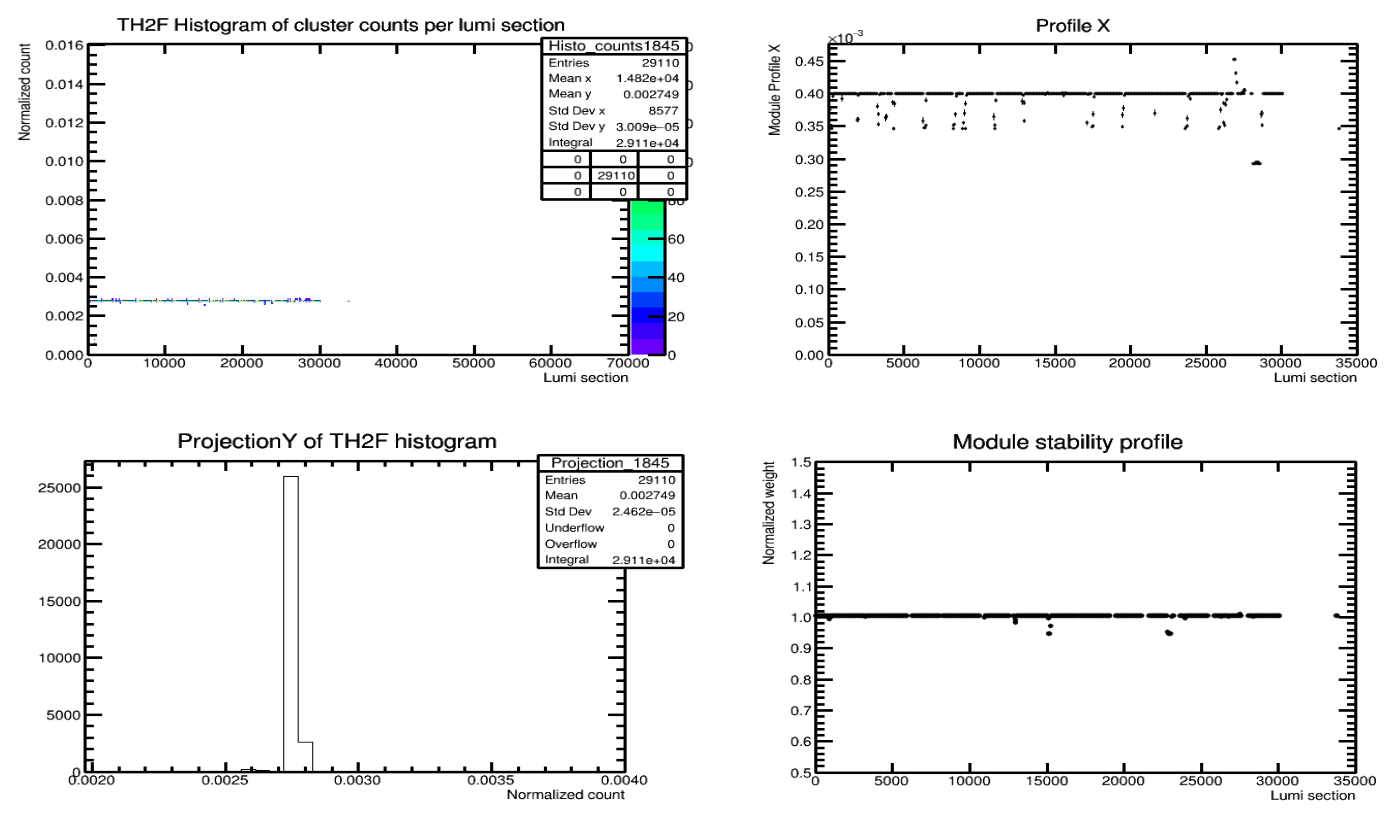
\includegraphics[width=0.9\textwidth]{ashish_thesis/Module_weight.png}
\caption{%
   Method to obtain module weights as a function of lumi section for categorizing good and bad modules. X profile of TH2F histogram (module PCC/total PCC per lumi section) is obtained. X profile is then filled in a TGraph after removing points with error $>$ 0.05. TGraph is normalized with the mean of Y projection of TH2F histogram to obtain module stability profile.
}
\label{fig:mod_weight}
\end{figure}


\begin{figure}[!htp]
\centering
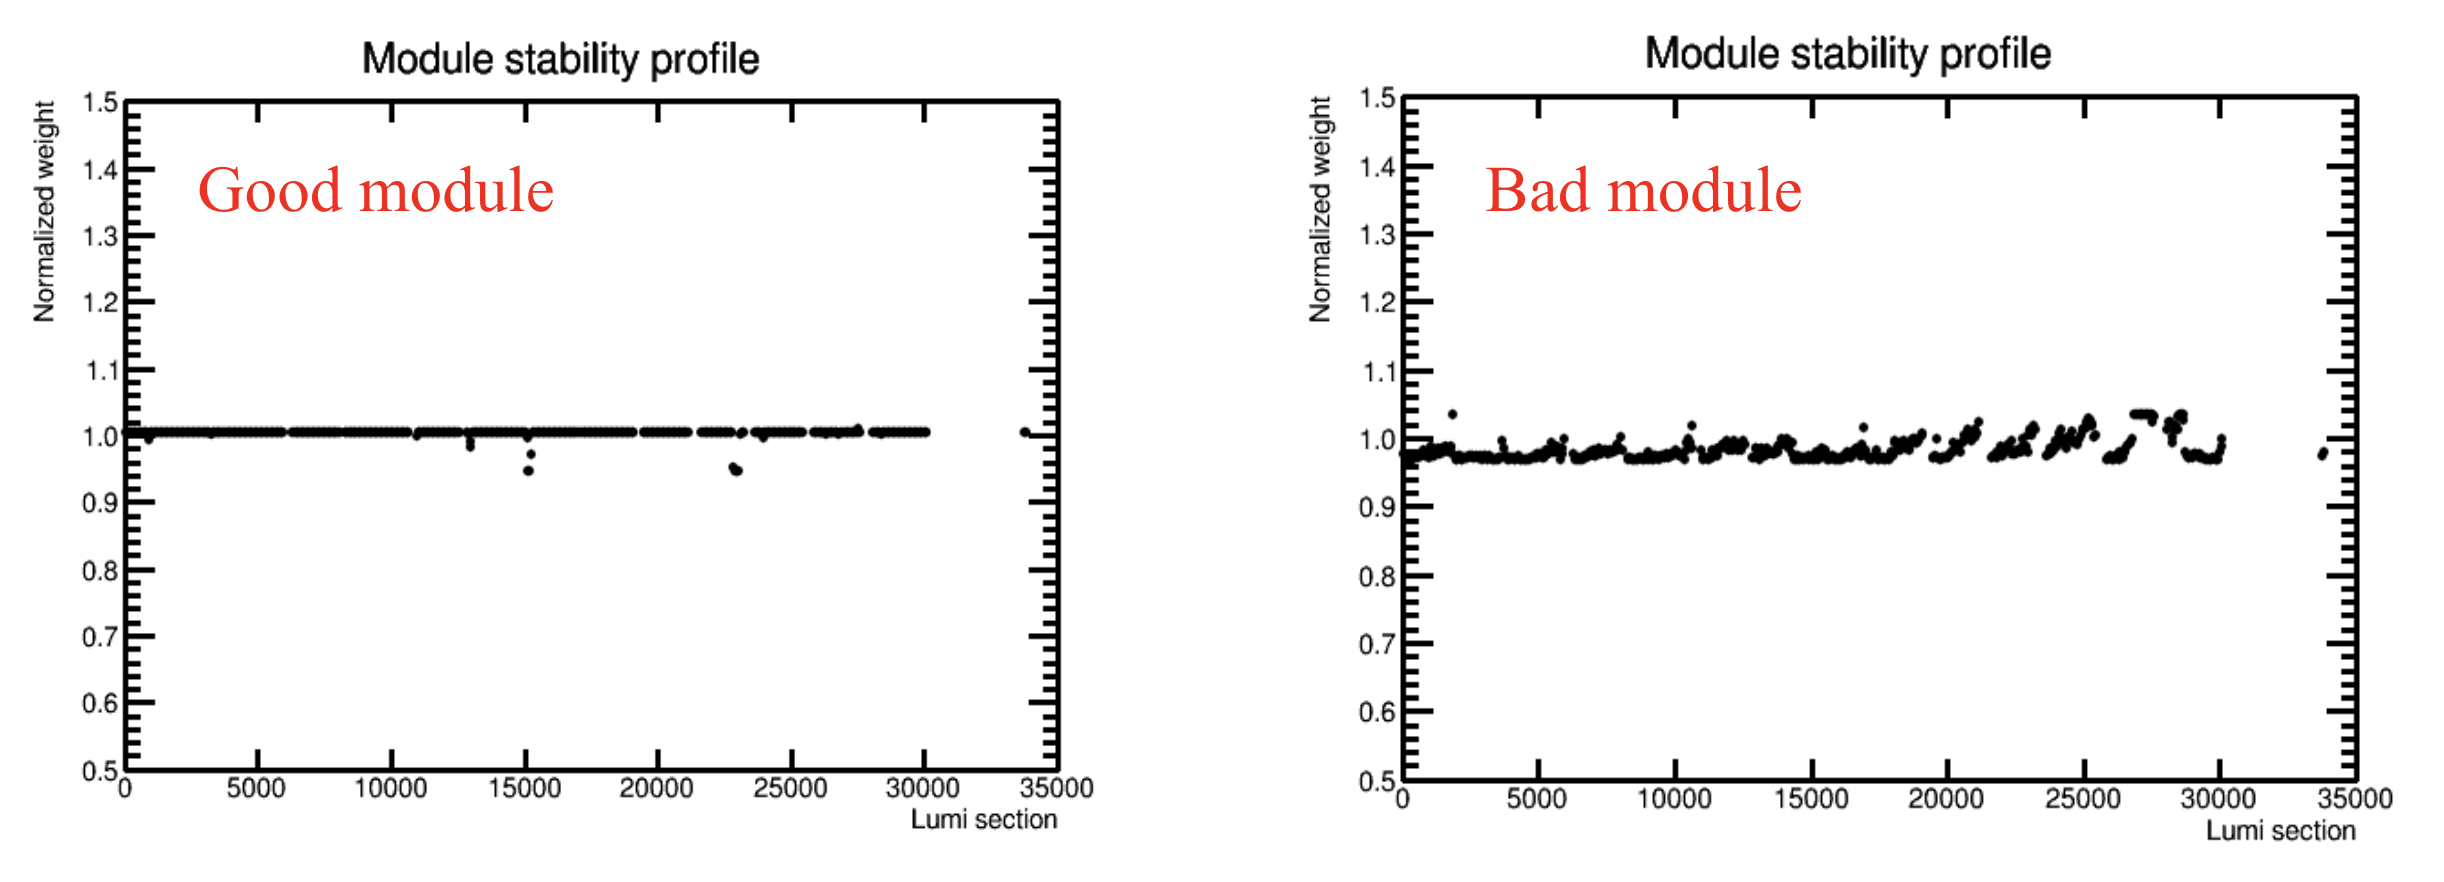
\includegraphics[width=1\textwidth]{ashish_thesis/good_bad_modules.png}
\caption{%
   Variation of normalized module weight with time. Modules showing significant change in module weight (shown in right figure) over time having large rms/mean values are used to make module vetolist.
}
\label{fig:goodbadmodules}
\end{figure}

Module vetolist is first created for period B, vdM Fill and then for other periods A, C, D1, D2, D3 and D4 as follows, 

Run 2018B and vdM Fill:
\begin{itemize}

\item Poor statistics lumi sections are removed by applying selection on total PCC Fig. \ref{fig:PCC_cut} and \ref{fig:f_it}.

\item All barrel layer 1 modules are removed as these modules are significantly affected by dynamic inefficiency effects, where the hit efficiency decreases at higher $L_{inst}$ due to the readout chip not being able to process all of the hits.                                                                              
\item A loose selection of 7\% based on rms/mean of module weight profile is applied where mean and rms values are obtained from y projection of module weight profile. Modules with significantly large rms/mean are removed with this loose selection as shown in Fig. \ref{fig:outliermodules}. 

\item Module stability is re-evaluated based on rms/mean values using an iterative method where in each step, appropriate selections are applied to remove bad modules until stable luminosity is attained as sshown in Fig. \ref{fig:sec_it_cut}.                                                      
\end{itemize}

Run 2018A, C and D:                                                                      
\begin{itemize}  

\item Period B module veto list is applied to these periods to determine remaining bad modules.

\item same procedure is used as period B. 

\item module weight comparisons between period B and these periods is done and modules with more than 3 sigma change in module weights are removed as shown in Fig. \ref{fig:mod_w_com} and Fig \ref{fig:mod_w_com_1}.      .                                                                             
\end{itemize}


\begin{figure}[!htp]
\centering
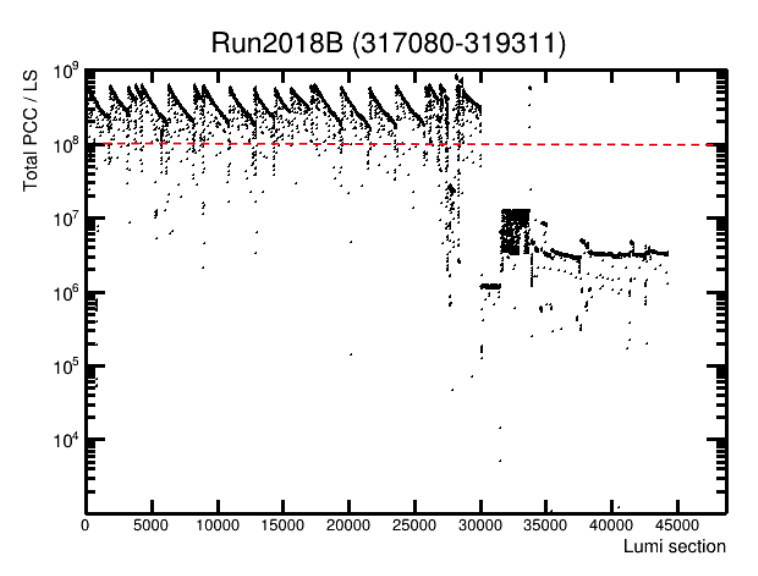
\includegraphics[width=0.7\textwidth]{ashish_thesis/Run2018B_totalPCC_cut.png}
\caption{%
 Total PCC as a function of lumi section for period 2018B.  Appropriate selection on total PCC is applied to remove low statistics lumi sections.
}
\label{fig:PCC_cut}
\end{figure}


\begin{figure}[!htp]
\centering
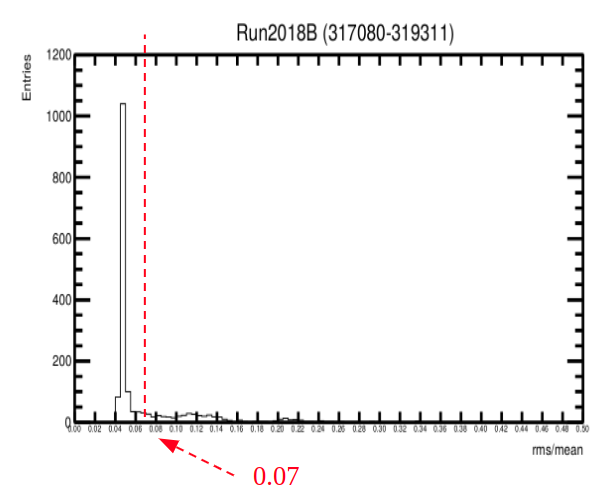
\includegraphics[width=0.7\textwidth]{ashish_thesis/first_iteration.png}
\caption{%
   A loose cut of 7\% is applied on rms/mean values of module stability profile to remove outlier modules.
}
\label{fig:f_it}
\end{figure}




\begin{figure}[!htp]
\centering
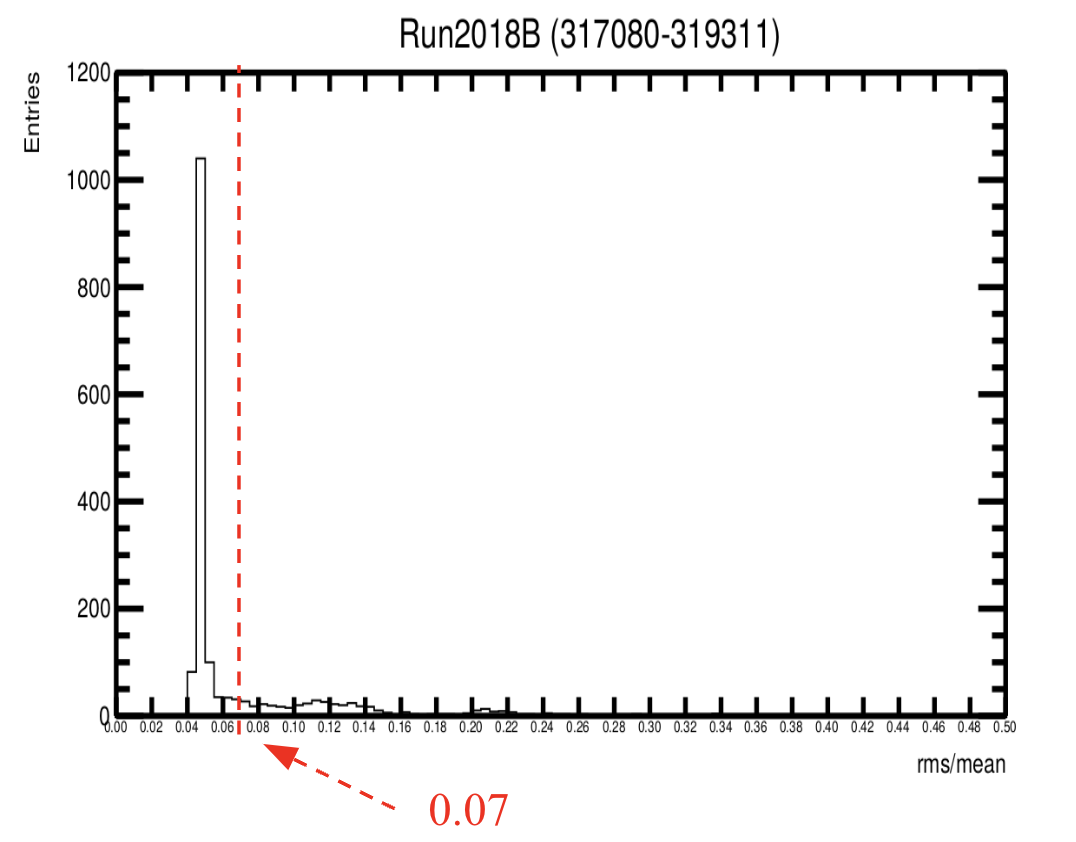
\includegraphics[width=0.8\textwidth]{ashish_thesis/cut_selection.png}
\caption{%
   RMS/mean of module weight profile for all modules. A loose selection of 7\% is applied to remove bad modules. Appropriate selections are applied in each iterative step to remove other bad modules.
}
\label{fig:outliermodules}
\end{figure}

\begin{figure}[!htp]
\centering
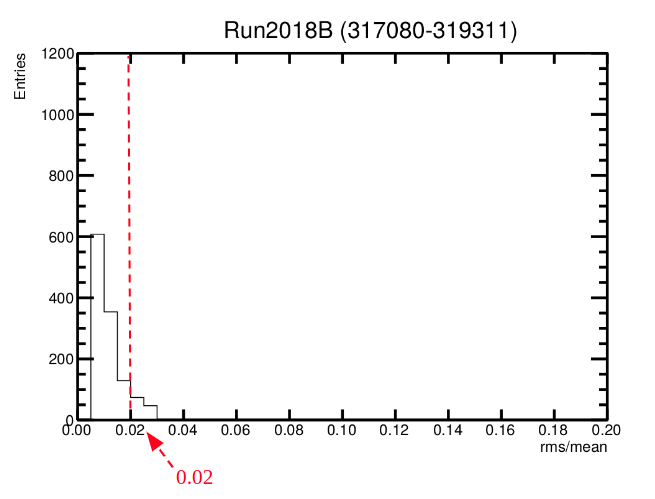
\includegraphics[width=0.7\textwidth]{ashish_thesis/second_iteration_cut.png}
\caption{%
 Final selection on RMS/mean of 2\% is applied to obtain module veto list for each period.
}
\label{fig:sec_it_cut}
\end{figure}


\begin{figure}[!htp]
\centering
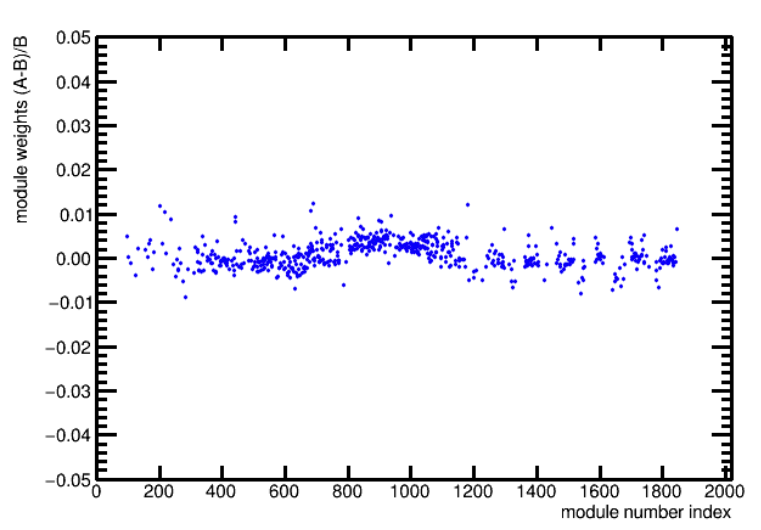
\includegraphics[width=0.7\textwidth]{ashish_thesis/mod_weight_comparison.png}
\caption{%
   Change in module weights between period A and B for all modules left after applying 2\% rms module vetolist.
}
\label{fig:mod_w_com}
\end{figure}



\begin{figure}[!htp]
\centering
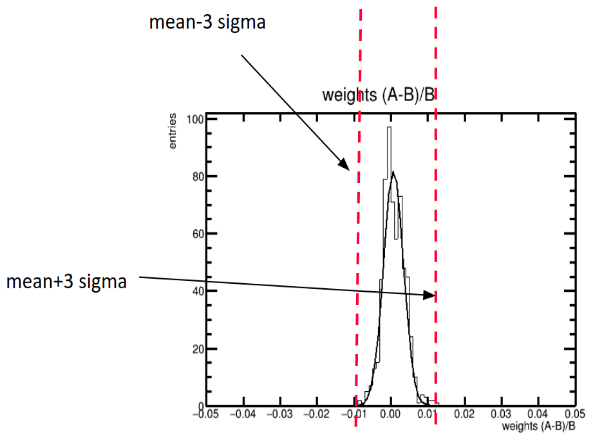
\includegraphics[width=0.8\textwidth]{ashish_thesis/mod_weight_comp_1.png}
\caption{%
   Projection of change in module weights between period A and B. Modules showing more than 3 sigma change are added to the module vetolist.
}
\label{fig:mod_w_com_1}
\end{figure}
   
 2\% selection on rms/mean of module weight profile gives the best stability for all pixel detector barrel layers and forward disks. Bad modules found after applying this 2\% selection in the final iterative step are used to constitute a 2 $\%$ rms module veto list for each period as shown in Table \ref{tab:per period veto}. 
                                                                                 
\begin{table}
  \begin{center}
    \begin{tabular}{ccccc}  
    \textbf{Period}   & \textbf{\# bad modules} & \textbf{\# good modules} \\ \hline
     2018A      &   1276   &  580    \\  
     2018B      &    802  &     1054  \\ 
     2018C      &   1076  &    780   \\ 
     2018D1     &  1169  &     687  \\ 
     2018D2     &  1184  &    672   \\ 
     2018D3     &  1081  &    775   \\ 
     2018D4     &  1032  &     824  \\ 
      \end{tabular}
    \caption{2 \% rms module vetolist for each period showing number of good and bad modules.}
    \label{tab:per period veto}
  \end{center}
\end{table}
 
To further improve the stability of PCC luminometer, $2\%$ rms common module vetolist is created as shown in Table \ref{tab:2commonveto}. Common module veto list is a combination of module veto list of all run periods A, B, C, D1, D2, D3 and D4. Approach to make a common module veto list is to start by combining module vetolists of period A,B and C, then combine A,B, C, D1 and so on. Less than $9\%$ of the pixel modules remain after applying module stability selections to be used for final luminosity measurement. 

\begin{table}
  \begin{center}
    \begin{tabular}{ccccc}  
    \textbf{Period}   & \textbf{\# bad modules} & \textbf{\# good modules} \\  \hline
     2018A + B + C      &  1417   &  439    \\  
     2018A + B + C + D1      &   1534  &   322    \\ 
     2018A + B + C + D1 + D2      &   1629 &    227   \\ 
     2018A + B + C + D1 + D2 + D3     &   1668 &   188    \\ 
     2018A + B + C + D1 + D2 + D3 + D4     &  1701 &     155  \\ 
      \end{tabular}
    \caption{2\% rms common module vetolist. This vetolist is created by combining module vetolists for each period.}
    \label{tab:2commonveto}
  \end{center}
\end{table}

The relative contribution to PCC luminosity from each pixel detector layer and disk after removing low statistics lumi sections and applying 2\% rms common module vetolist is shown in Fig. \ref{fig:stabprof}.


\begin{figure}[!htp]
\centering
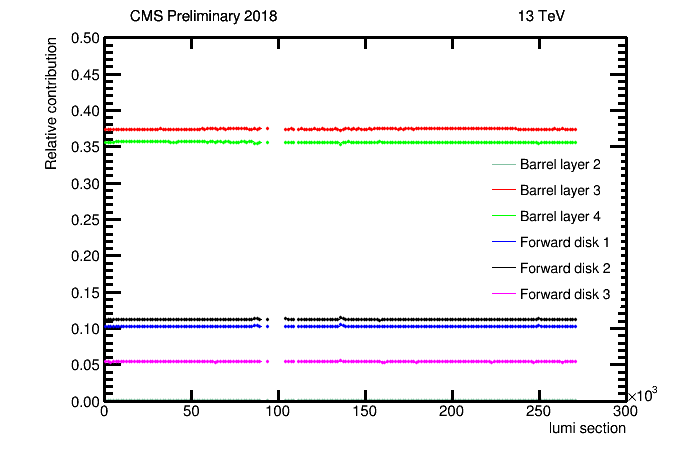
\includegraphics[width=0.8\textwidth]{ashish_thesis/ProfileX_combined_testing_LUM_20-001.png}
\caption{%
   Stability profiles of pixel detector layer and disk modules for 2\% rms common module vetolist.
}
\label{fig:stabprof}
\end{figure}

%\subsection{Reasons for the inclusion of certain modules in the veto list}

The module veto list in particle physics experiments is a list of detector modules that are excluded from the analysis of data due to their known or suspected high rate of background events or other issues that could affect the accuracy of the measurement. The inclusion of certain modules in the veto list is based on various factors, including:

\begin{itemize}

\item Radiation damage: The harsh radiation environment in the LHC can cause damage to the silicon pixel sensors over time, leading to increased leakage currents, noise, or reduced charge collection efficiency.

\item Manufacturing defects: Defects in the silicon material or issues during the manufacturing process can result in poorly performing pixel modules. These defects may not be immediately evident but can become more pronounced over time.

\item Electronic noise: Noisy electronic components or crosstalk between channels can lead to an increased number of false signals or noise in the pixel module data.

\item Temperature variations: Temperature fluctuations can affect the performance of the pixel modules, leading to changes in their noise levels, gain, or charge collection efficiency.

\item High voltage issues: Problems with the high voltage supply to the pixel modules can result in unstable operation, leading to erratic behavior or complete module failure.

\item Partial module failure: A pixel module may suffer from partial failure, with some pixels or readout channels not functioning properly. This can lead to an increased number of dead or noisy pixels in the module.

\item Readout or data acquisition issues: Errors in the readout electronics or data acquisition system can lead to data corruption or loss, affecting the performance of the pixel modules.

\item Calibration issues: Inaccurate or outdated calibration parameters can result in incorrect measurements, leading to the appearance of abnormal behavior in the pixel module data.

\item Firmware or software issues: Bugs in the firmware or software responsible for controlling and reading out the pixel modules can lead to abnormal behavior or incorrect measurements.

\item Mechanical or alignment issues: Mechanical stresses or misalignments during the installation or operation of the pixel detector can affect the performance of the pixel modules or cause them to fail.

\item Contamination or environmental factors: Contamination of the pixel modules by dust, moisture, or other substances can affect their performance or cause them to fail. Similarly, external environmental factors, such as magnetic fields or vibrations, can impact the operation of the pixel modules.

\end{itemize}

The inclusion of certain modules in the veto list is based on a careful analysis of the detector performance and the expected background rates in a given experiment. By excluding modules with high background rates or other issues, the analysis can be improved and the accuracy of the measurement can be increased.


\section{Afterglow corrections}

Type 1 and Type 2 afterglow corrections are essential for obtaining accurate PCC measurements. Type 1 afterglow noise, also known as electronic spillover, is caused by the long waveform of the signal in silicon. On the other hand, Type 2 afterglow noise is the exponentially decaying detector activation due to the production of secondary particles when high-energy particles interact with the detector material as shown in Fig. \ref{fig:pcc_afterglow}. Afterglow noise is corrected by creating a model of the afterglow tail of a single colliding bunch, which is then normalized to the luminosity of the colliding bunch crossing. A bunch-by-bunch histogram containing bunch trains undergoes afterglow correction, where the afterglow model is multiplied with the luminosity of each colliding bunch pair and subsequently subtracted from all following bunches. This correction process is performed iteratively for all colliding bunch pairs, ensuring that a given bunch crossing is fully corrected before being used to correct the subsequent bunch crossings. The afterglow correction, or scale factor, is calculated by taking the ratio of the corrected and uncorrected PCC. This scale factor is then applied to individual bunch-by-bunch histograms in the zero bias data. In addition to afterglow corrections, pedestal correction is another important aspect to consider. Pedestal correction refers to the adjustment of baseline values in the detector readout to account for any systematic offsets or drifts. This process involves measuring the detector's output when no signal is present and subtracting this baseline value from the measured signal during data collection. By performing pedestal correction, the accuracy and stability of the detector's measurements are significantly improved, contributing to more reliable PCC measurements.

%Type 1 and 2 afterglow corrections are measured and applied to the PCC measurement. Type 1 afterglow noise is electronic spillover due to long waveform of the signal 549 in silicon and Type 2 afterglow noise is exponentially decaying detector activation due to production of secondary particles when high energy particles interact with detector material as shown in Fig. 15. Afterglow noise is corrected by making a model of afterglow tail of a single colliding bunch, normalized to the luminosity of the colliding bunch crossing. Bunch-by-bunch histogram containing bunch trains is corrected for afterglow where afterglow models is multi554 plied with the luminosity of each colliding bunch pair and subtracted from all following bunches. This correction is performed iteratively over all colliding bunch pairs such that a given bunch crossing is fully corrected before it is used to correct the succeeding bunch crossings. The afterglow correction (or scale factor) can be calculated by taking the ratio of corrected and uncorrected PCC. This scale factor is applied to individual bunch-by-bunch histograms in the zero bias data.

\begin{itemize}

\item Type 1 afterglow correction: Type 1 afterglow refers to the residual signals in the detector caused by particles from previous bunch crossings. These particles can be trapped in the detector's sensitive volume, leading to an overestimation of the actual number of pixel clusters. The Type 1 afterglow correction aims to correct for this by subtracting the expected contribution of these residual signals from the raw PCC data.

\item Type 2 afterglow correction: Type 2 afterglow is associated with the activation of detector material due to high-energy particle interactions. When high-energy particles interact with the detector material, they can cause the material to become radioactive. The decay of these radioactive isotopes produces additional signals in the detector, which can lead to an overestimation of the number of pixel clusters. The Type 2 afterglow correction aims to account for these additional signals by subtracting the expected contribution of the activation-induced background from the raw PCC data.

\item Pedestal afterglow correction: The pedestal afterglow refers to the baseline noise level in the detector, which can be influenced by factors such as temperature fluctuations, electronic noise, and radiation damage. This noise can cause an over- or underestimation of the actual number of pixel clusters. The pedestal afterglow correction aims to correct for this by adjusting the raw PCC data based on a measurement of the pedestal noise level.

\end{itemize}


\begin{figure}[!htp]
\centering
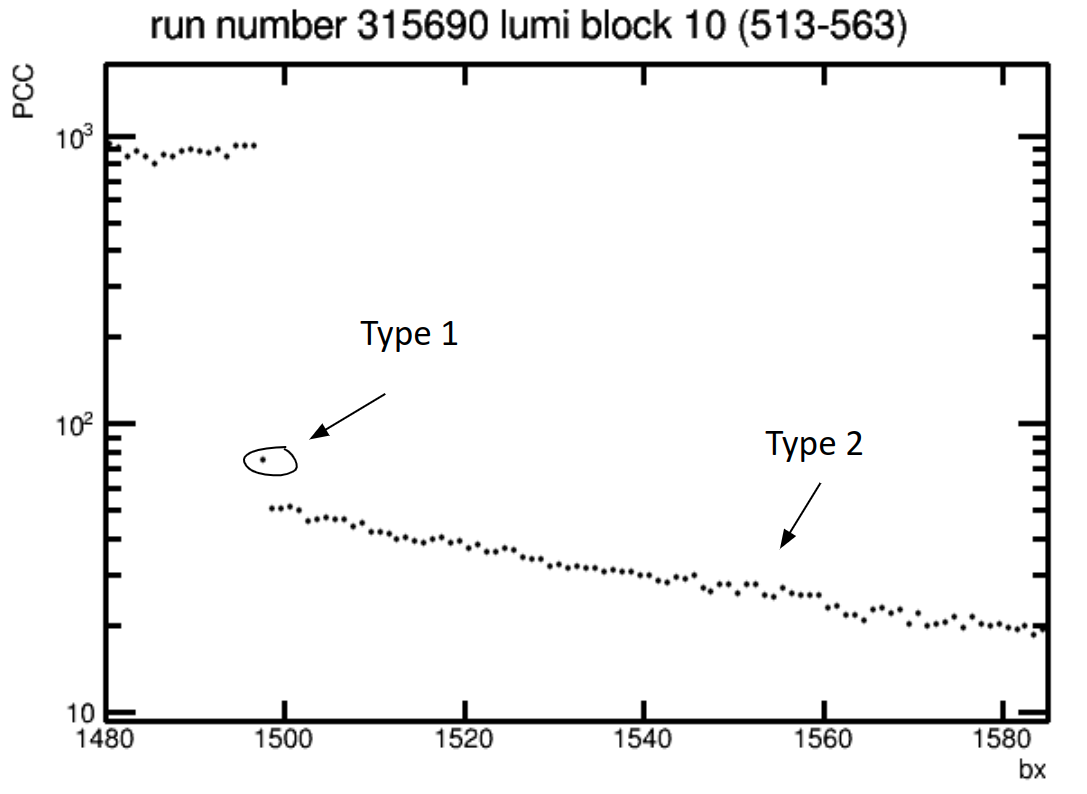
\includegraphics[width=0.7\textwidth]{ashish_thesis/afterglow_type1_type2.png}
\caption{%
Afterglow corrections are calculated from cluster rate measurements in empty bunches. Electronic spillover (“Type-1”). Type-1 noise is due to long waveform of the signal in silicon. First empty bunch after bunch train is used to calculate it. Exponentially decaying detector activation (“Type-2”).  Type-2 noise is due to production of secondary particles when high energy particles interact with detector material. All empty bunches after bunch train are used to calculate it.
}
\label{fig:pcc_afterglow}
\end{figure}






